% Template for ICIP-2015 paper; to be used with:
%          spconf.sty  - ICASSP/ICIP LaTeX style file, and
%          IEEEbib.bst - IEEE bibliography style file. cambio para probar adsfasfasfasfsf
% --------------------------------------------------------------------------
\documentclass[spanish,twocolumn]{article}
\usepackage{spconf,amsmath,graphicx}
\usepackage{mathptmx}
\usepackage{mathtools}
\usepackage{amsmath}
\usepackage{mathrsfs}
\usepackage{amssymb}
\usepackage{amsfonts}
\usepackage[utf8]{inputenc}
\usepackage{babel}
\usepackage{color}
\usepackage[Algoritmo]{algorithm}
\usepackage{algpseudocode}
\usepackage{multicol}
\usepackage{caption,setspace}
\usepackage{subfig}
\usepackage{graphicx}

\algrenewcommand\algorithmicif{\textbf{si}}
\algrenewcommand\algorithmicend{\textbf{fin}}
\algrenewcommand\algorithmicfor{\textbf{para}}
\algrenewcommand\algorithmicdo{\textbf{hacer}}
\algrenewcommand\algorithmicwhile{\textbf{mientras}}
\algrenewcommand{\algorithmicrequire}{\textbf{Entrada:}}
\algrenewcommand{\algorithmicensure}{\textbf{Salida:}}
\selectlanguage{spanish}
% Example definitions.
% --------------------
\def\x{{\mathbf x}}
\def\L{{\cal L}}

% Title.
% ------
\title{OPTIMIZACIÓN MULTIOBJETIVO BASADA EN LA SINTONIZACIÓN DE LOS PARÁMETROS DE CLAHE PARA OBTENER DISTINTOS NIVELES DE CONTRASTE EN IMÁGENES MÉDICAS}
%\title{OPTIMIZACIÓN MULTIOBJETIVO PARA LA MEJORA DEL CONTRASTE BASADA EN CLAHE.}
%
% Single address.
% ---------------
\name{Luis G. Moré, Marcos A. Brizuela, Horacio Legal Ayala, Diego Pinto-Roa, José Luis Vázquez Noguera}
\address{Facultad Politécnica - Universidad Nacional de Asunción}
%
% For example:
% ------------
%\address{School\\
%	Department\\
%	Address}
%
% Two addresses (uncomment and modify for two-address case).
% ----------------------------------------------------------
%\twoauthors
%  {A. Author-one, B. Author-two\sthanks{Thanks to XYZ agency for funding.}}
%	{School A-B\\
%	Department A-B\\
%	Address A-B}
%  {C. Author-three, D. Author-four\sthanks{The fourth author performed the work
%	while at ...}}
%	{School C-D\\
%	Department C-D\\
%	Address C-D}
%
\begin{document}
%\ninept
%
\maketitle
%
\begin{abstract}
In certain medical images, it is possible to achieve a contrast enhancement at different levels, in order to highlight different structures present therein. This could be useful to medical specialists to perform more specific diagnoses. Tuning parameters Contrast Limited Adaptive Histogram Equalization is proposed, using a multi-objective metaheuristic. The proposed objectives are to maximize the amount of information available (via Entropy) and minimize distortion in the resulting images (Structural Similarity Index) simultaneously. The results show a set of solutions or Pareto Front, which represents the image with different contrast levels and different levels of commitment between Entropy and Structural Similarity Index, which shows that these are contradictory.
%La mejora del contraste en imágenes médicas presenta desafíos importantes, debido a que se necesita realzar los detalles y también preservarlos, de forma a que la mejora sea de ayuda para análisis posteriores. Se propone un enfoque de mejora multiobjetivo basada en CLAHE, utilizando SMPSO como metaheurística, además de la Entropía y el SSIM como objetivos, de manera a maximizar el contraste y minimizar la distorsión de los resultados. Se obtienen distintos niveles de contraste en imágenes de radiografía del tórax, y así se resaltan distintos detalles de éstas. Los resultados obtenidos se analizan con ayuda de un especialista de manera a determinar la utilidad del enfoque, además se verifica que los objetivos son contradictorios.
\end{abstract}
%
\begin{keywords}
SMPSO, CLAHE, Entropía, SSIM, Mejora del Contraste, Optimización.
\end{keywords}
%
\section{INTRODUCTION}
\label{sec:intro}

It is very important to perform the Improvement of medical imaging contrast character, because this way it is possible to emphasize and maintain the features present in them. Radiographs have specific characteristics contrast, as in the case of chest x-rays and mammograms, which may be differences in notorious contrast due to the attenuation of characteristics X Rays \cite{chang1998image}.

There are several proposals Contrast Enhancement Histogram-based transformations \cite{1658094}. Local improvement approaches prove to be extremely useful when enhance details in medical images, and there are various proposals that focus on improving contrast radiographs  \cite{1625082,4712472,5360176}. In our a proposed metaheuristic optimization objectives, so tune the input parameters of the algorithm improvement described in section \ref{sec:clahe} contrast, so you get a group of contrasting images, which will be evaluated will be used as the provided gain and distortion introduced by the equalization (section \ref{sec:metricas}) information. Images are generated with Images with different relationships between contrast and distortion, in order to highlight different features of the test images, which is useful for analysis the accomplished by the specialist.

In the literature there are proposals for improvement based on metaheuristics, as shown in \cite{Hashemi20101816}, in which Genetic algorithms are used in \cite{morebrizuela2014} a proposal similar to the approach used, although it focuses on a single objective and only one result is obtained for each original image, or \cite{Shanmugavadivu2014243}, where multi-objective metaheuristic also is used; the main difference is that our proposal is implemented more effectively in medical imaging because CLAHE shows satisfactory results in this type of images \cite{reza2004,5360176}, and show the best results automatically .

The rest of the paper is organized as follows: In section \ref{sec:clahe} the contrast enhancement algorithm is described briefly adopted; in section n \ref{sec:metricas} is used the metrics for evaluating results; in section n \ref{sec:formulacion} formally poses the problem being solved; Section \ref{sec:propuesta} shows the optimization How applies to contrast enhancement algorithm; then the sectional area \ref{sec:resultadosdiscusion}, the results are discussed, and finally in the section area \ref{sec:conclusion} the corresponding conclusions are detailed. 


\section{Contrast Limited Adaptive Histogram Equalization}
\label{sec:clahe}

This contrast enhancement approach presented in  \cite{Zuiderveld:1994:CLA:180895.180940} is an extension of the original algorithm Adaptive Histogram Equalization (AHE) \cite{pizer1987adaptive}; in both Methods Histogram implements an equalization based on Contextual Regions whose dimensions are defined by $(\mathcal{R}_x, \mathcal{R}_y)$ to perform equalization in several areas of the image. Inconsistencies between borders of the image are corrected using bilinear interpolation. AHE amplification presents problems of noise, then in CLAHE a limitation is implemented in the contrast through limiting the number of pixels that can attain a certain level of gray within the local histogram; Here {\it Clip Limit} coefficient $\mathcal{C}$ is defined as a factor that is closely related to the contents of the histogram.

%Este enfoque de mejora de contraste presentado en \cite{Zuiderveld:1994:CLA:180895.180940} es una extensión del algoritmo original Adaptive Histogram Equalization (AHE) \cite{pizer1987adaptive}; en ambos métodos se implementa una Ecualización del Histogama basada en {\it Regiones Contextuales} cuyas dimensiones están delimitadas por $(\mathcal{R}_x, \mathcal{R}_y)$, para realizar la ecualización en varios sectores de la imagen. Las inconsistencias entre fronteras de la imagen se corrigen aplicando interpolación bilineal. AHE presenta problemas de amplificación del ruido, entonces en CLAHE se implementa una limitación en el contraste a través de la limitación de la cantidad de pixeles que pueden alcanzar cierto nivel de gris dentro del histograma local; aquí se define el coeficiente {\it Clip Limit} $\mathcal{C}$ como un factor que está fuertemente relacionado con los contenidos del histograma. %Si definimos un coeficiente $\mathcal{C}$ relativamente bajo, entonces los histogramas de las regiones contextuales no muestran picos, por lo que se obtiene una mejora del contraste relativamente suave. Si definimos un $\mathcal{C}$ alto, obtenemos un comportamiento de $CLAHE$ que resulta ser equivalente al algoritmo $AHE$. En el contexto del trabajo propuesto, la selección de parámetros de CLAHE es fundamental para lograr resaltar los detalles en radiografías, y evitar una amplificación en el ruido indeseable \cite{pisano1998}.

\section{METRICS EVALUATION}
\label{sec:metricas}

For each result obtained by CLAHE, you need to use metrics to quantify the quality of the resulting images; this is why we adopted two coefficients that are important for comparisons between results.  

\subsection{Entropía}
\label{ssec:entropia}

The {\it Entropía de la Información} is a measure of randomness present in the image \cite{tsai2008information}. You can define the Entropy of the image as:

\begin{equation}\label{eq:entropia}
\mathscr{H}=-\sum_{i=0}^{L-1}\mathcal{P}_i log_2(\mathcal{P}_i) [bits] \quad \mathscr{H} \in {0,..,log_2(L)} 
\end{equation}

Where $\mathcal{P}_i$ is the probability of occurrence of grays level $i$ in the histogram and $L$ is the maximum gray level that can be used to represent the image. This metric is interesting because it is strongly associated with the average brightness of the image \cite{108593}; this ratio helps us see how the contrast increases as a result of the transformation of the image.

\subsection{Structural similarity index}
\label{ssec:ssim}

The {\it Structural Similarity Index (SSIM)} \cite{wang2004image} is an index that measures the degree of distortion in a resulting image $T$ as a result of applying a Contrast Enhancement to the original image $I$. SSIM is calculated by block, so if $I_x$ and $T_y$ define two windows to the original and resulting images, respectively, the SSIM is defined as shown below:

\begin{equation}\label{eq:ssim}
\resizebox{.9\hsize}{!}
{
$SSIM(I,T)=\frac{(2\mu_{I_x}\mu_{T_y}+C_1)(2\sigma_{I_xT_y}+C_2)}{(\mu_{I_x}^2+\mu_{T_y}^2+C_1)(\sigma_{I_x}^2+\sigma_{T_y}^2+C_2)} \quad SSIM \in [0,1]$
}
\end{equation}

Where $\mu_{I_x}$ is the average intensities of $I_x$; $\mu_{T_y}$ is the average of intensities of $T_y$; $\sigma_{I_x}^2$ and $\sigma_{T_y}^2$ are the intensity variances and $I_x$ and $T_y$, respectively; $\sigma_{I_x T_y}$ is the covariance between $I_x$ and $T_y$; $C_1=(K_1L^2)$, $L$ is the dynamic range of intensities of the pixels (256 for a grayscale image of 8 bits) and $K_1 \ll 1$ is a small constant; $C_2=(K_2 L)^2$, y $K_2 \ll 1$; and $K_2 \ll 1$; both $C_1$ y $C_2$ are constants that are used to stabilize the division in case the denominator approaches zero.


Donde $\mu_{I_x}$ es el promedio de intensidades de $I_x$; $\mu_{T_y}$ es el promedio de intensidades de $T_y$; $\sigma_{I_x}^2$ y $\sigma_{T_y}^2$ son las varianzas de intensidades de $I_x$ e $T_y$, respectivamente; $\sigma_{I_x T_y}$ es la covarianza entre $I_x$ e $T_y$; $C_1=(K_1L^2)$, $L$ es el rango dinámico de intensidades de los pixeles (256 para una imagen en escala de grises de 8 bits) y $K_1 \ll 1$ es una constante pequeña; $C_2=(K_2 L)^2$, y $K_2 \ll 1$; tanto $C_1$ y $C_2$ son constantes que se usan para estabilizar la division en caso de que el denominador tienda a cero.

\begin{algorithm}[H]
    \scriptsize
    \begin{algorithmic}[1]
        \Require imagen de entrada $I$, número de partículas $\Omega$, número de iteraciones $t_{max}$
        \State Inicializar los parámetros $\omega$, $C_1$, $C_2$, $t=0$, $lower\_limit_1$, $lower\_limit_2$, $lower\_limit_3$, $upper\_limit_1$, $upper\_limit_2$, $upper\_limit_3$, $\mathscr{X}$
        %\For{cada $i$-ésima partícula del enjambre}
        %    \State Inicializar la posición $x_i$ aleatoriamente
        %    \State Inicializar la velocidad $v_i$ a 0
        %    \State ${imagenMejorada}$ = CLAHE(${x_i}$, ${imagenOriginal}$)
        %    \State ${f_i}$ = evaluarAptitud(${imagenOriginal}$, ${imagenMejorada}$)
        %    \State Establecer el mejor individual inicial $p_i$ por el valor inicial $x_i$
        %    \If{$f_i < f_{p_g}$}
        %        \State reemplazar $p_g$ por el valor de $x_i$
        %    \EndIf
        %\EndFor
        \While{$t$ $<$ $t_{max}$}
            \For{cada $i$-ésima partícula del enjambre}
                \State Calcular la nueva velocidad de la partícula $\overrightarrow{v_i}^t$ utilizando la ecuación \eqref{eq:psobasico2}, sujeto a las restricciones impuestas por \eqref{eq:restricciondelta}

%                \begin{equation*}\label{eq:psobasico2}
%                    \overrightarrow{v_i}(t) = \omega \cdot \overrightarrow{v_i} \cdot (t-1) + C_1 \cdot r_1 \cdot (\overrightarrow{x_{p_i}}-\overrightarrow{x_i}) + C_2 \cdot r_2
%                \end{equation*}



                \State Calcular la nueva posición de la partícula $\overrightarrow{x_i}^t$ con la expresión de posición \eqref{eq:psobasico}
                %\begin{equation*}\label{eq:psobasico}
                %    \overrightarrow{x_i}(t) = \overrightarrow{x_i}(t-1) + \overrightarrow{v_i}(t)
                %\end{equation*}

                \State ${T}$ = CLAHE(${\overrightarrow{x_i}^t}$, ${I}$)
                \State ${f^t_i}$ = $f(I, \overrightarrow{x_i}^t)$%evaluarAptitud(${I}$, ${T}$)
                \If{$f^t_i < f_{\overrightarrow{x}_{p_i}}$}
                    \State reemplazar $\overrightarrow{x}_{p_i}$ por el nuevo valor de $\overrightarrow{x_i}^t$
                \EndIf
                \If{$ \overrightarrow{x_i} \succ \overrightarrow{x_{g_i}}$  }
                    \State actualizar $\mathscr{X}$
                \EndIf
                \State $t$ = $t$ + 1
            \EndFor
        \EndWhile
    \Ensure $\mathscr{X}$
    \end{algorithmic}
    \caption{Algoritmo $PSO-CLAHE$ Multiobjetivo.}
    \label{alg:pso_clahe}
\end{algorithm}

\section{FORMULATION OF THE PROBLEM POSED}
\label{sec:formulacion}

Given the input image $I$, and a vector $\overrightarrow{x}=(\mathcal{R}_x, \mathcal{R}_y, \mathcal{C})$, where $\mathcal{R}_x$ and $\mathcal{R}_y$ form the contextual region and $\mathscr{C}$ is the ClipLimit, calculate the desired set of $\mathscr{X}$ solutions simultaneously maximizing the objectives $f_1$ and $f_2$, as shown below:

\begin{equation}\label{eq:fitness}
    f(I, \overrightarrow{x}) = \{ f_1(I, \overrightarrow{x}), f_2(I, \overrightarrow{x}) \} \qquad f_1,f_2 \in [0,1]
\end{equation}

where:
\begin{itemize}
%\item $\overrightarrow{x}=(\mathcal{R}_x, \mathcal{R}_y, \mathcal{C})$, donde $\mathcal{R}_x$ y $\mathcal{R}_y$ conforman la región contextual y $\mathscr{C}$ es el Clip Limit.
\item $f_{1}(I, \overrightarrow{x})=\frac{\mathscr{H}(T)}{log_{2}L}$ es la Entropía normalizada de la imagen $T$.%, y $L$ la cantidad de grises disponibles.
\item $f_{2}(I, \overrightarrow{x})=SSIM(I,T)$ es el Índice de Similitud Estructural entre $I$ y $T$.

Siendo $T$ la imagen mejorada por $CLAHE(\overrightarrow{x},I)$ con los parámetros dados por $\overrightarrow{x}$ aplicados a $I$.

\end{itemize}

sujeto a:

\begin{itemize}
\item $\mathcal{R}_x \in [2,..,M]$ en los números $\mathbb{N}$.
\item $\mathcal{R}_y \in [2,..,N]$ en los números $\mathbb{N}$.
\item $\mathscr{C} \in (0,1]$ en los números $\mathbb{R}$.
\end{itemize}

Ésto significa que los valores de $\mathcal{R}$ solamente pueden tomar valores enteros positivos entre $(2,2)$ y $(M,N)$ y que $\mathscr{C}$ puede tomar un valor mayor a cero y menor o igual a 1.


\section{propuesta}
\label{sec:propuesta}

$SMPSO$ \cite{4938830} algorithm is used, where potential solutions $\overrightarrow{x}=(\mathcal{R}_x, \mathcal{R}_y, \mathcal{C})$ {\it partículas} called and the set $\Omega$ is called {\it enjambre}. Each particle $\overrightarrow{x_i}$ is updated at each generation according to $t$ following equation:

\begin{equation}\label{eq:psobasico}
\overrightarrow{x_i}^t = \overrightarrow{x_i}^{(t-1)} + \overrightarrow{v_i}^t
\end{equation}

where the factor $\overrightarrow{v_i}$ known as speed and is given by:
%donde el factor $\overrightarrow{v_i}$ se conoce como la velocidad y está dado por:

\begin{equation}\label{eq:psobasico2}
\overrightarrow{v_i}^t = \omega \cdot \overrightarrow{v_i}^{(t-1)} + C_1 \cdot r_1 \cdot (\overrightarrow{x_{p_i}}-\overrightarrow{x_i}) + C_2 \cdot r_2 \cdot (\overrightarrow{x_{g_i}}-\overrightarrow{x_i})
\end{equation}

Aquí, $\overrightarrow{x_{p_i}}$ es la mejor solución que encontró $\overrightarrow{x_i}$, $\overrightarrow{x_{g_i}}$ es la mejor partícula (también conocida como {{\it líder}) que se encuentra en todo el enjambre, $\omega$ es el peso de la inercia de la partícula, $r_1$ y $r_2$ son dos números aleatorios, y $C_1$ y $C_2$ son son parámetros que controlan el efecto de las partículas locales  y globales. Si una partícula es mejor que otra, se dice que la $domina$, y la dominancia está definida de la siguiente manera: $\overrightarrow{x_{g_i}} \succ \overrightarrow{x_i}$ si y sólo si

\begin{equation}\label{eq:dominanciapareto}
         \begin{cases}  f_i(I,\overrightarrow{x_{g}})  \geq f_i(I,\overrightarrow{x}) \forall i \in \{1,2\} \\
                        f_i(I,\overrightarrow{x_{g}}) > f_i(I,\overrightarrow{x}) \exists i \in \{1,2\} \\
         \end{cases}
\end{equation}

El {\it Conjunto Pareto} es el grupo de soluciones $\mathscr{X}$, y la imagen en el espacio objetivo es el {\it Frente Pareto}.

In addition, a restriction in $SMPSO$ $\overrightarrow{v}$, for each component $j$ $\overrightarrow{x}$, according to the following equation is performed:

                
\begin{equation}\label{eq:restricciondelta}
    v_{i,j}^t = \begin{cases}  delta_j &\mbox{if } v_{i,j}^t > delta_j \\
                                -delta_j & \mbox{if } -delta_j \\
                                v_{i,j}^t & otherwise \end{cases}
\end{equation}

where: 
\begin{equation} \label{eq:restricciondelta2}
delta_j= \frac{upper\_limit_j - lower\_limit_j}{2}
\end{equation}

\textbf{Algoritmo \ref{alg:pso_clahe}} shows how the proposal is implemented. The resulting images are evaluated according to the metric \eqref{eq:entropia} y \eqref{eq:ssim}, and the best results are obtained based on these metrics form a Pareto front of solutions. The front shows a series of images with different contrast levels, so as to highlight particular characterıstics it.

And the interaction between particles $CLAHE$ $SMPSO$ shown in \textbf {Fig. 1}. Parameters CLAHE receives as input the values stored by a particle $(\mathcal{R}_x,\mathcal{R}_y, \mathscr{C})$ and the original image $I$, and the processed image is $SSIM$ calculated metric $\mathscr{H}$ and so as to obtain the objective functions. The non-dominated solutions are stored in the pareto front. This process is repeated until a stopping criterion defined.


%La interacción entre CLAHE y las partículas de SMPSO se muestran en la \textbf {Fig. 1}. CLAHE recibe como parámetros de entrada los valores almacenados por una partícula $(\mathcal{R}_x,\mathcal{R}_y, \mathscr{C})$ y la imagen original $I$, y a la imagen procesada se le calculan las métricas $\mathscr{H}$ y $SSIM$ de manera a obtener las funciones objetivo. Las soluciones no dominadas se almacenan en el conjunto pareto. Éste proceso se repite hasta alcanzar un criterio de parada definido.

\begin{minipage}[b]{1.0\linewidth}
  \vspace{0.5cm}
  \centering
  \centerline{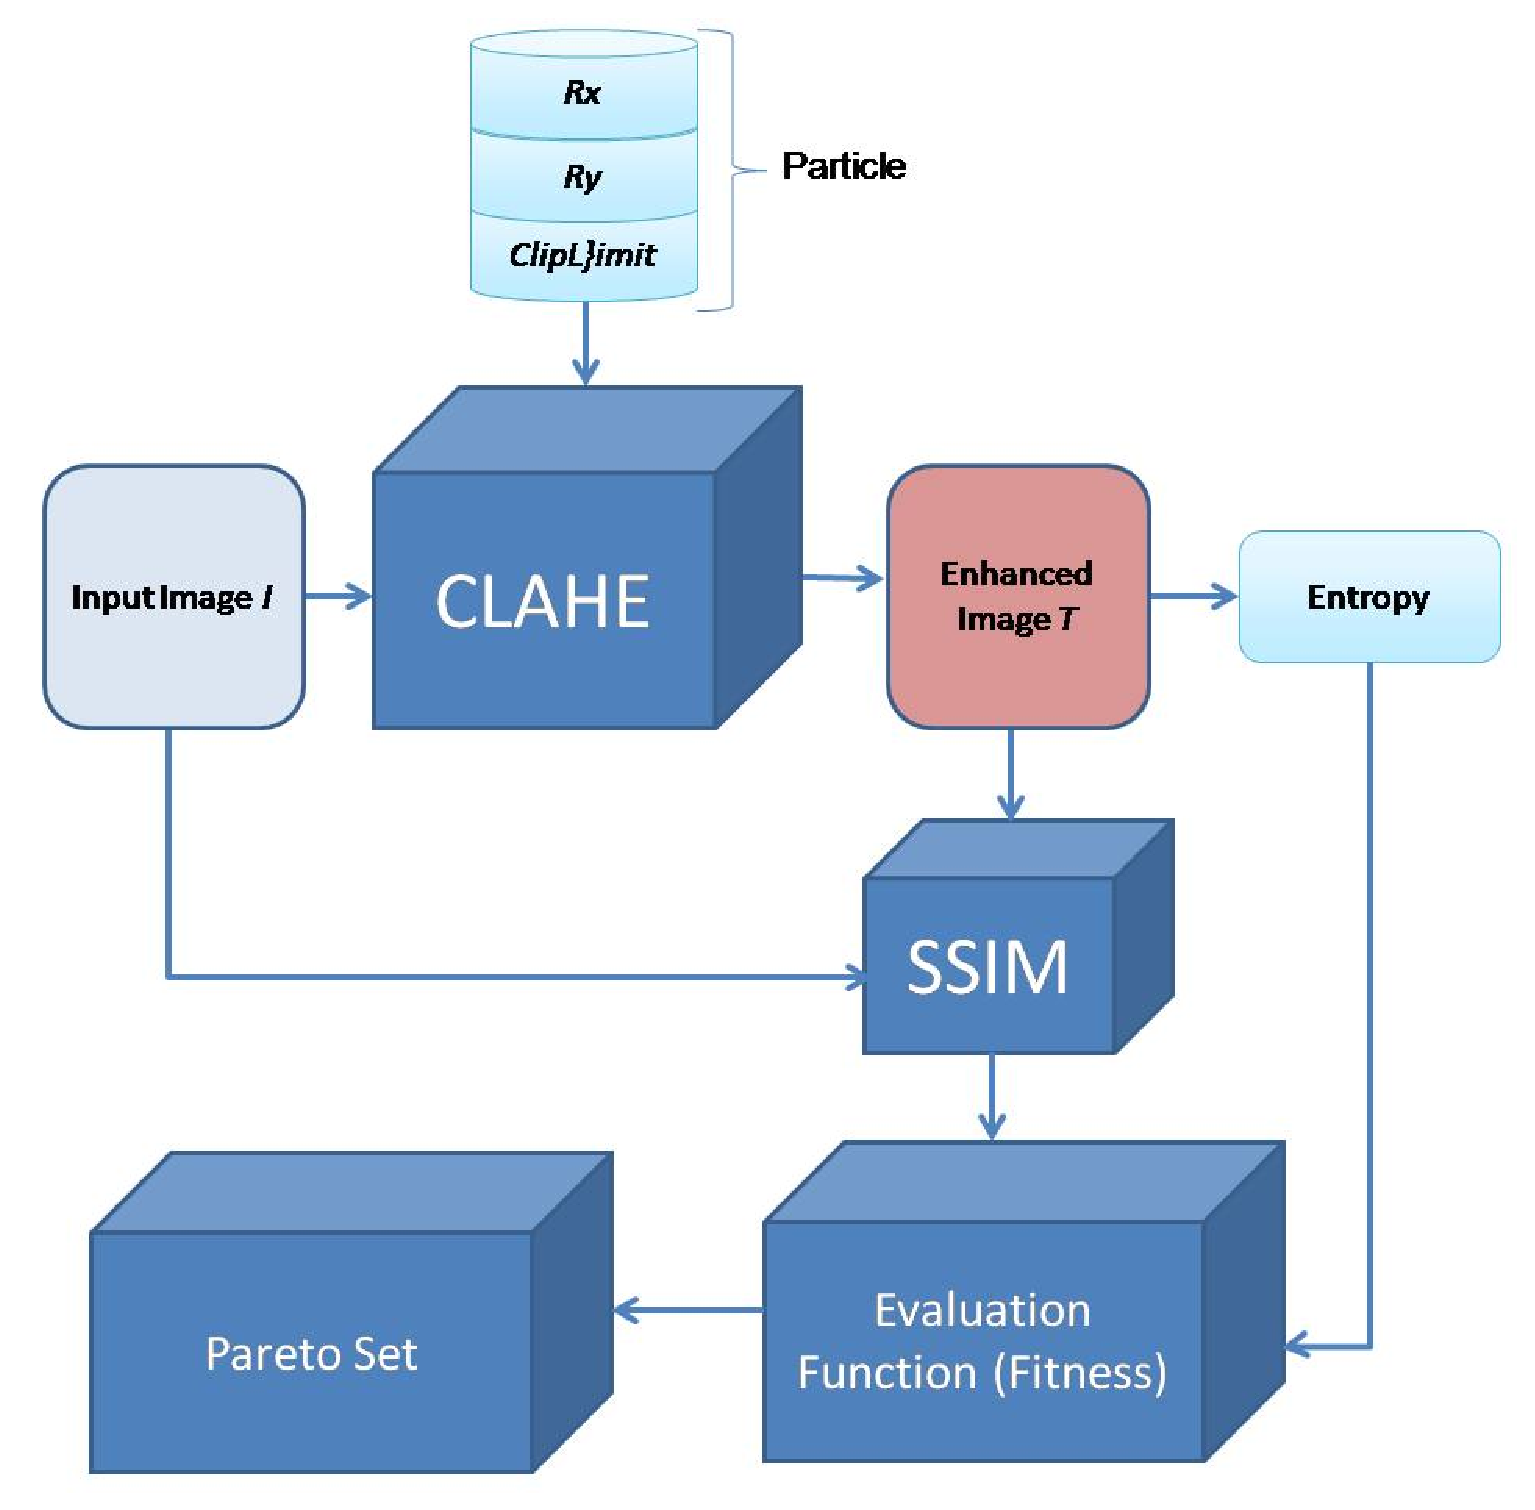
\includegraphics[height=6.5cm]{Figures/particula_clahe2}}
  \vspace{0.5cm}
  \label{fig:particula_clahe}
  \captionof{figure}{Interacción entre CLAHE y SMPSO.}
\end{minipage}

\section{resultados y discusión}
\label{sec:resultadosdiscusion}

The tests were performed using an Intel Core i3 dual core laptop, with 2.5GB RAM and Windows 7 32 bits. $SMPSO$ implementation is available at \cite{5586354}, meanwhile the corresponding implementations of $CLAHE$ and $\mathscr{H}$ y $SSIM$ are available at \cite{opencv_library}. Tests were performed using 16 images of chest radiograph and mammography, in order to assess the effectiveness of this proposal; they were downloaded from http://openi.nlm.nih.gov/. The initial parameters chosen for $SMPSO$ are listed in \textbf{Table \ref{table:parametrospso}}:

%Para la ejecución se utilizó como hardware una laptop con procesador Intel Core i3 de doble núcleo, con 2,5 GB de memoria RAM, y sistema operativo Windows 7 de 32 bits. La metaheurística $SMPSO$ está disponible en \cite{5586354}; mientras que la implementación de $CLAHE$ y de las métricas $\mathscr{H}$ y $SSIM$ se encuentran en \cite{opencv_library}. Se realizaron pruebas contra {\color{red} 16} imágenes de radiografía del tórax y mamografías, de manera a comprobar la efectividad de la propuesta; las mismas se descargaron del sitio http://openi.nlm.nih.gov/.  Se escogieron parámetros iniciales como se muestra en la \textbf{Table \ref{table:parametrospso}}:


%Para la ejecución se utilizó como hardware una laptop con procesador Intel Core i3 de doble núcleo, con 2,5 GB de memoria RAM, y sistema operativo Windows 7 de 32 bits. La metaheurística $SMPSO$ está disponible en \cite{5586354}; mientras que la implementación de $CLAHE$ y de las métricas $\mathscr{H}$ y $SSIM$ se encuentran en \cite{opencv_library}. Se realizaron pruebas contra {\color{red} 16} imágenes de radiografía del tórax y mamografías, de manera a comprobar la efectividad de la propuesta; las mismas se descargaron del sitio http://openi.nlm.nih.gov/.  Se escogieron parámetros iniciales como se muestra en la \textbf{Table \ref{table:parametrospso}}:

\begin{table}[h]
\begin{center}
 \begin{tabular}{||c c | c c||} 
 \hline
 Parametro & Valor & Parametro & Valor \\ [0.5ex] 
 \hline\hline
 $lower\_limit_{\mathscr{R}_x}$ & $2$ & $upper\_limit_{\mathscr{R}_x}$ & $M/2$ \\ 
 \hline
 $lower\_limit_{\mathscr{R}_y}$ & $2$ & $upper\_limit_{\mathscr{R}_y}$ & $N/2$ \\  
 \hline
 $lower\_limit_{\mathscr{R}_{\mathscr{C}}}$ & $0$ & $upper\_limit_{\mathscr{R}_{\mathscr{C}}}$ & $0,5$ \\
\hline
$\Omega$ & $100$ & $t$ & $100$ \\ 
\hline
$C_1$ $min$ & $1,5$ & $C_1$ $max$ & $2,5$ \\ 
\hline
$C_2$ $min$ & $1,5$ & $C_2$ $max$ & $2,5$ \\ 
\hline
$r_1$ $min$ & $0,0$ & $r_1$ $max$ & $1,0$ \\ 
\hline
$r_2$ $min$ & $0,0$ & $r_2$ $max$ & $1,0$ \\ [1ex]
\hline
\end{tabular}
\end{center}
\caption[Parámetros de entrada para $SMPSO$]{Initial parameters for $SMPSO$}
\label{table:parametrospso}
\end{table}
 
 30 executions of $SMPSO-CLAHE$ were performed for every test image. Aproximately 300 pareto solutions were obtained for every image, which represents a wide group of images at different levels of contrast and distortion, thereby facilitating further analysis. In \textbf {Fig. 2}  and \textbf {Fig. 3} there are 2 of the pareto set solutions, in order to visually assess how contrast varies, and also the original image as reference. In \textbf {Fig. 4} it is noteworthy that there is an inverse relationship between objectives, this is, when $\mathscr{H}$ is increased, the $SSIM$ coefficient decreases; this means that both metrics are complementary in order to mantain the compromise between contrast enhancement and distortion minimization. From the pareto set it is possible to obtain images which allow to visualize different details while the contrast changes. It is also remarkable that the soft tissues are better seen in chest radiographs when certain contrast is reached (see \textbf {Fig.} 2c). A similar effect is achieved in mammograms (see \textbf {Fig.} 3b), in which potential injuries are more visible, but the fine details are preserved successfully. In this proposal, a significal amount of resulting images are obtained, with different relations between contrast and distortion, in an automatic manner, which represents an advantage because it avoids configuring tuning parameters arbitrarily, as in \cite{1419470}.


\section{conclusiones}
\label{sec:conclusion}
A metaheuristic algorithm is presented which maximizes simultaneously contrast by means of Entropy and Structural Similarity Index; with the latter it is possible to minimize image distortion, in medical imagery context, especifically in chest radiographs and mammograms. Experimental results show a set of solutions at different contrast levels, and allowing to highlight different structures. This would allow medical specialists to handle different visualization options automatically, which might be useful for diagnostics.

The authors are very enthusiastic about the results obtained with this proposa, and are still executing tests with several images found in the search engine. As future work it might be useful to adopt new metaheuristics, such as multiobjective genetic algorithms.





% Below is an example of how to insert images. Delete the ``\vspace'' line,
% uncomment the preceding line ``\centerline...'' and replace ``imageX.ps''
% with a suitable PostScript file name.
% -------------------------------------------------------------------------
%\begin{figure}[t]

%\begin{minipage}[b]{1.0\linewidth}
%  \centering
%  \centerline{\includegraphics[width=8.5cm]{Figures/image1}}
%  \vspace{2.0cm}
%  \centerline{(a) Result 1}\medskip
%\end{minipage}
%
%\begin{minipage}[b]{.48\linewidth}
%  \centering
%  \centerline{\includegraphics[width=4.0cm]{Figures/image3}}
%  \vspace{1.5cm}
%  \centerline{(b) Results 3}\medskip
%\end{minipage}
%\hfill
%\begin{minipage}[b]{0.48\linewidth}
%  \centering
%  \centerline{\includegraphics[width=4.0cm]{Figures/image4}}
%  \vspace{1.5cm}
%  \centerline{(c) Result 4}\medskip
%\end{minipage}
%
%\caption{Example of placing a figure with experimental results.}
%\label{fig:res}
%
%\end{figure}


% To start a new column (but not a new page) and help balance the last-page
% column length use \vfill\pagebreak.
% -------------------------------------------------------------------------
%\vfill
%\pagebreak

% References should be produced using the bibtex program from suitable
% BiBTeX files (here: refs). The IEEEbib.bst bibliography
% style file from IEEE produces unsorted bibliography list.
% -------------------------------------------------------------------------
\onecolumn
\noindent\begin{minipage}[b]{1.0\linewidth}
  \centering
   
   \begin{minipage}[t]{0.3\linewidth}  
   		\centering
        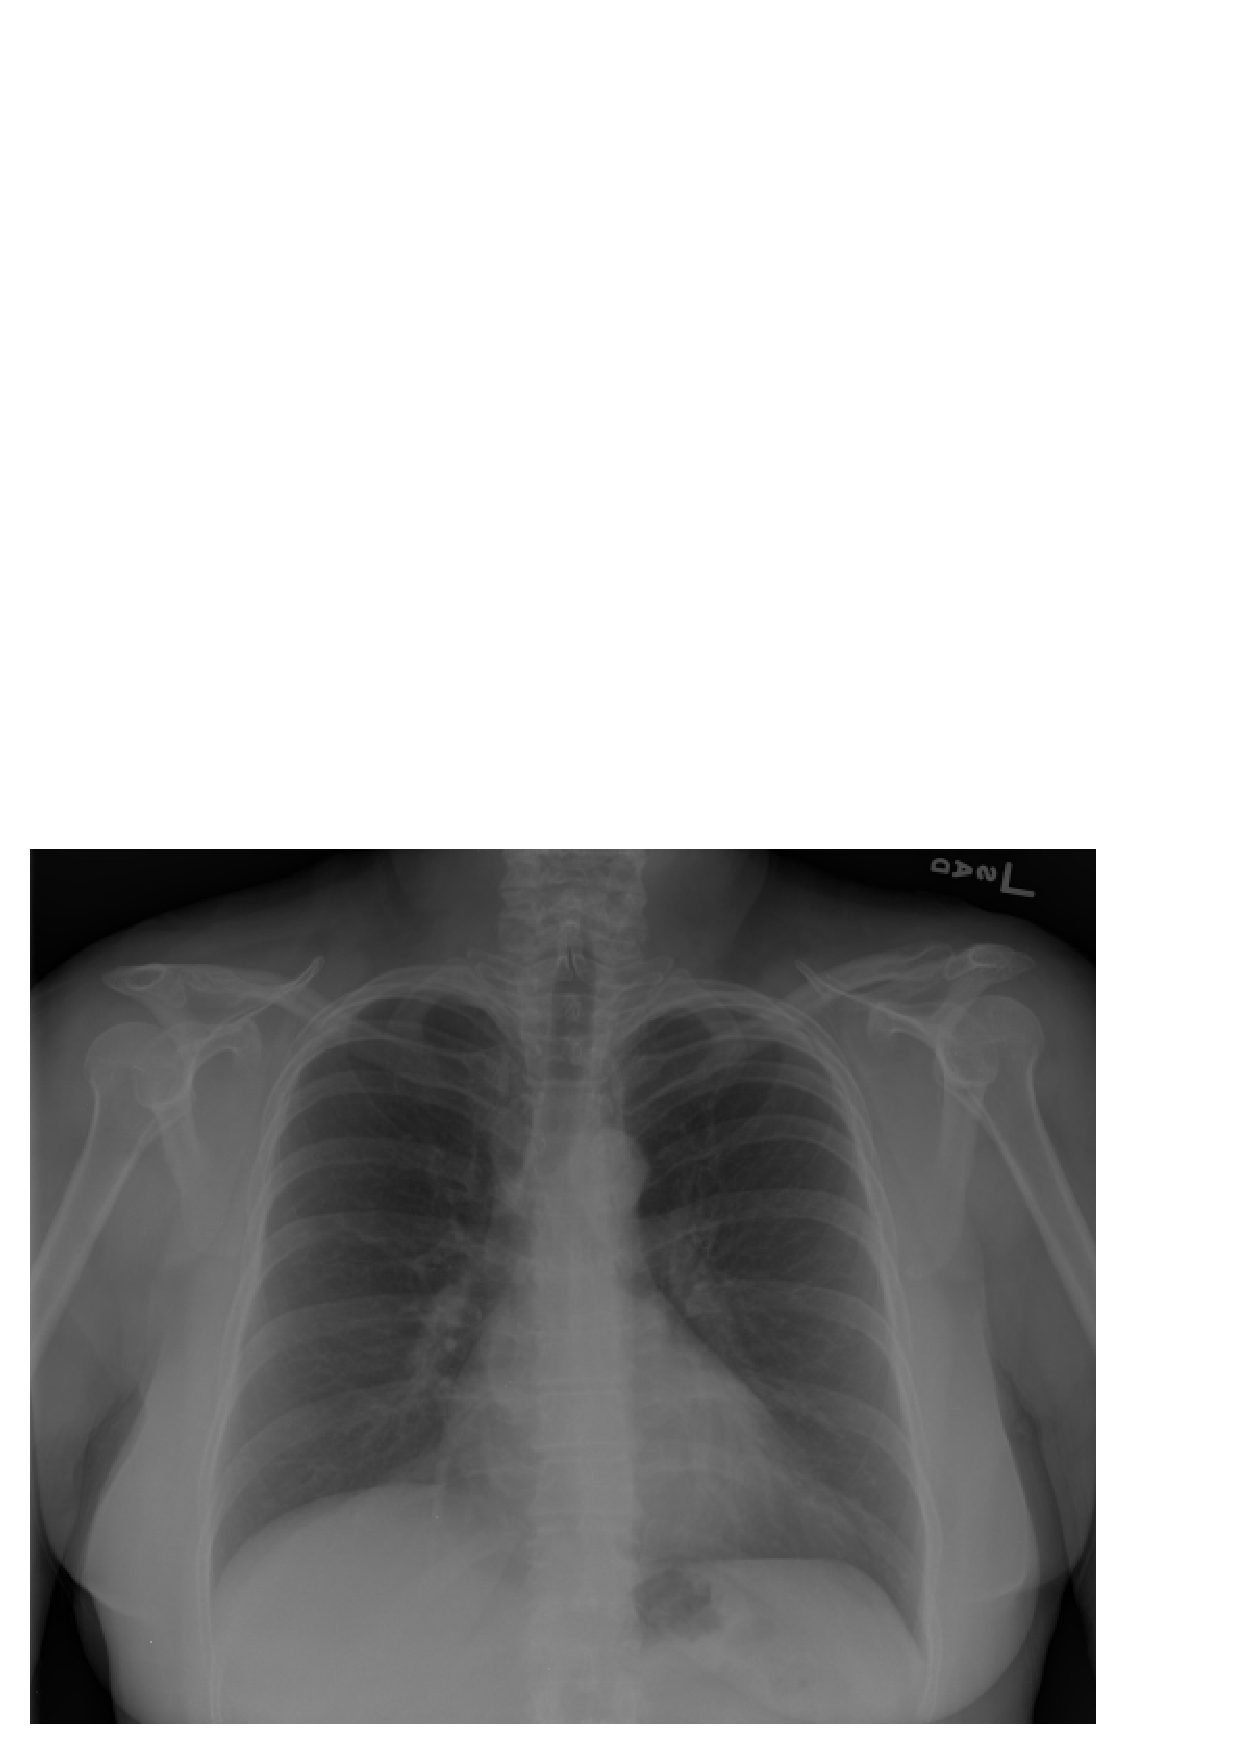
\includegraphics[width=4cm]{Figures/100_IM-0002-1001.png}
   		\captionof{subfigure}{Imagen original}
  	\end{minipage}
  \hspace{1pt}
   \begin{minipage}[t]{0.3\linewidth}  
   		\centering
        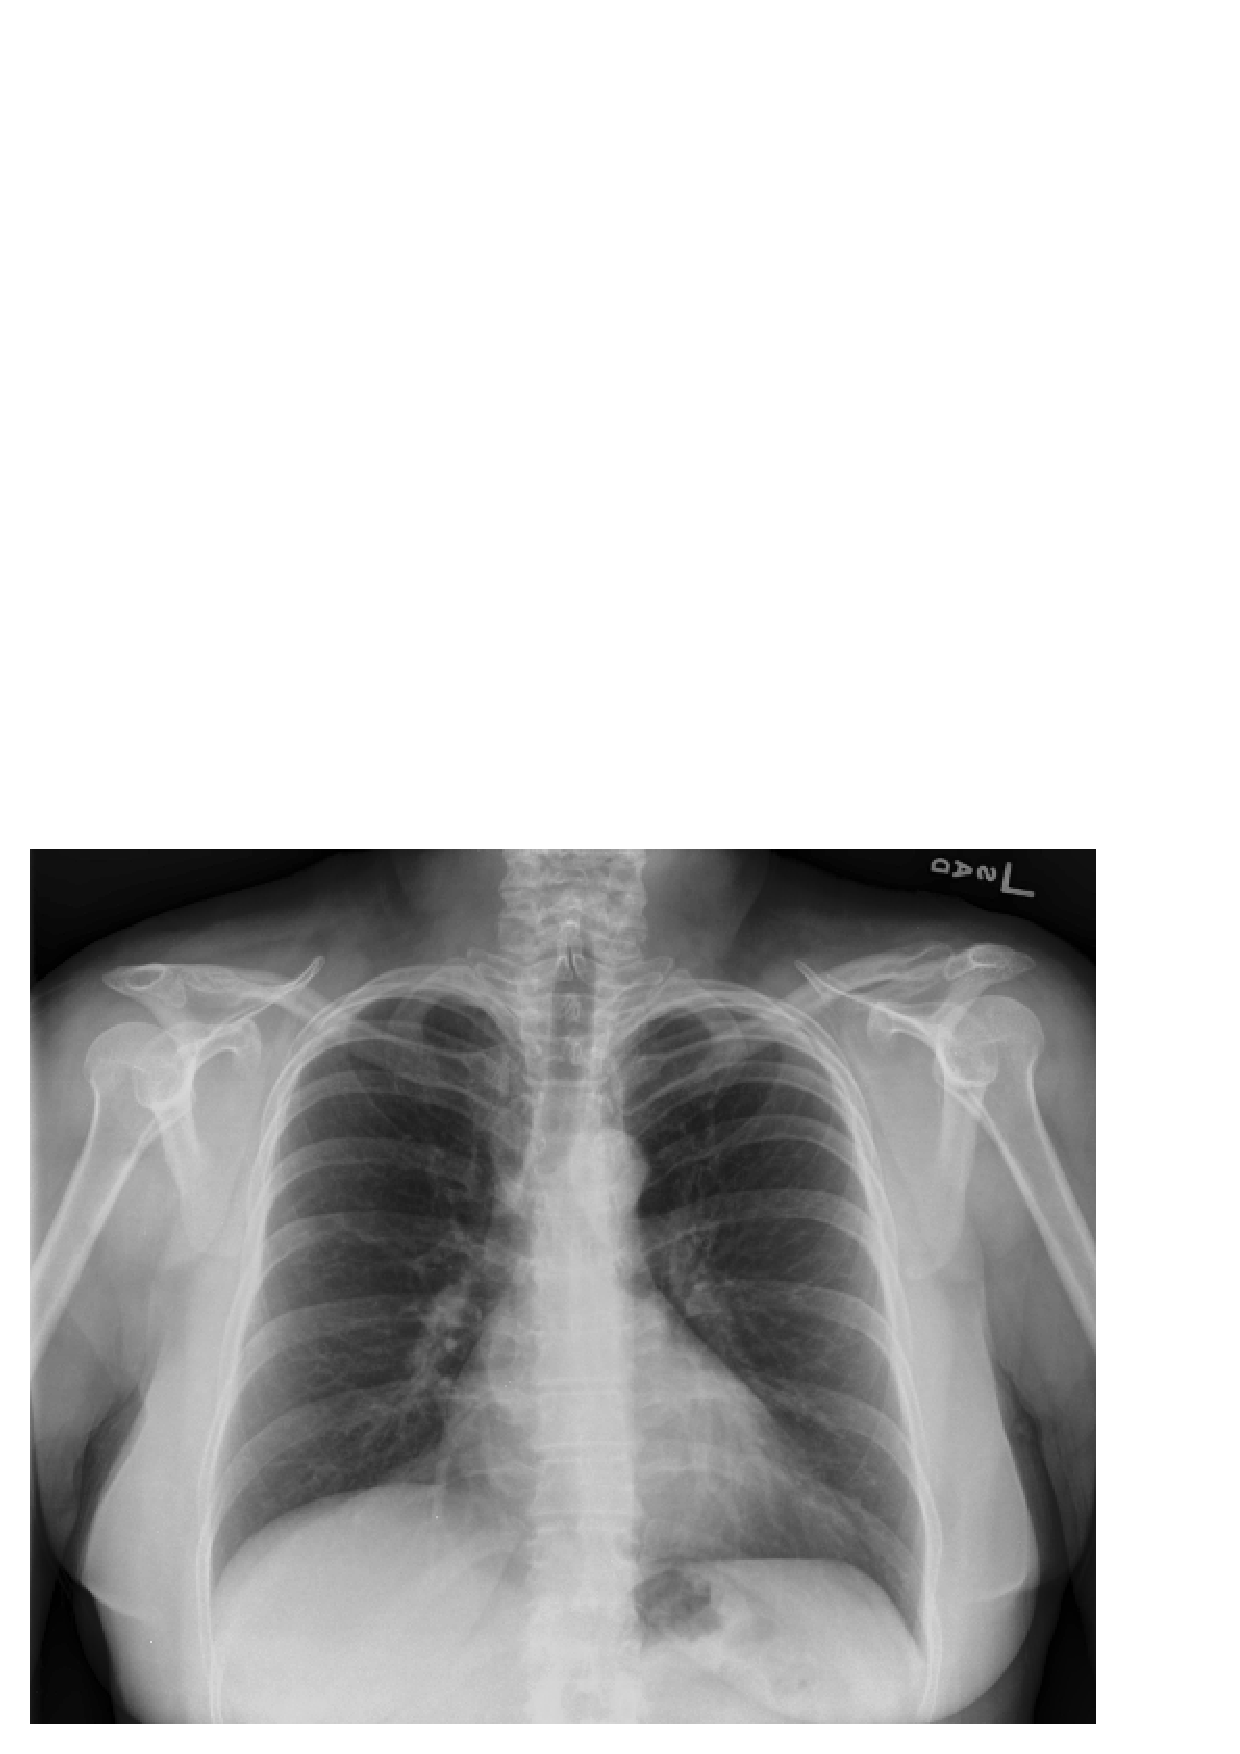
\includegraphics[width=4cm]{Figures/1182-100_IM-0002-1001.png}
   		\captionof{subfigure}{Imagen resultante. $SSIM=0.9688$ $\mathscr{H}=0.7922$}
  	\end{minipage}
  \hspace{1pt}
   \begin{minipage}[t]{0.3\linewidth}  
   		\centering
        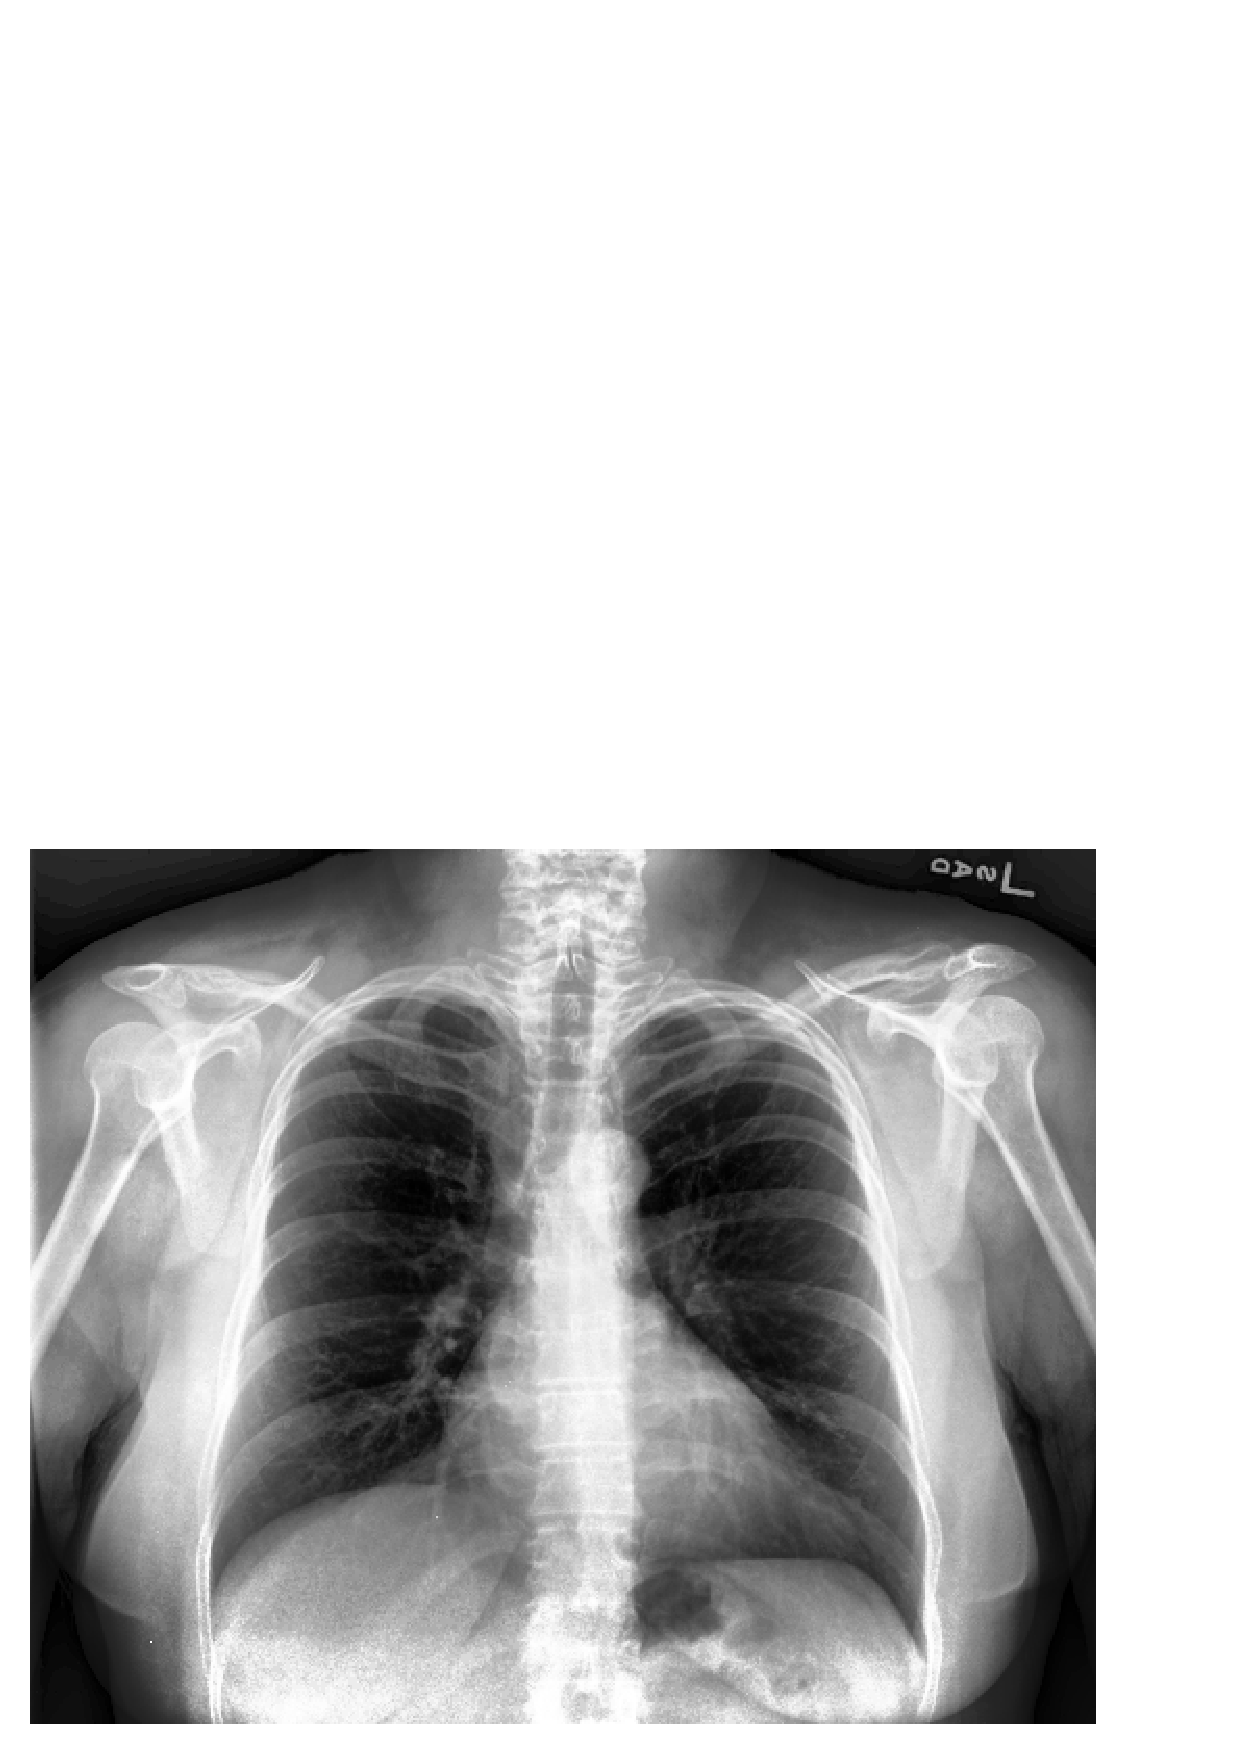
\includegraphics[width=4cm]{Figures/738-100_IM-0002-1001.png}
   		\captionof{subfigure}{Imagen resultante. $SSIM=0.6530$ $\mathscr{H}=0.9933$}
  	\end{minipage}
  \vspace{0.5cm}
    \label{fig:resultado1}
  \captionof{figure}{Resultados de PSO-CLAHE multiobjetivo. }

\end{minipage}

\begin{minipage}[b]{1.0\linewidth}
  
   \begin{minipage}[t]{0.3\linewidth}  
   		\centering
        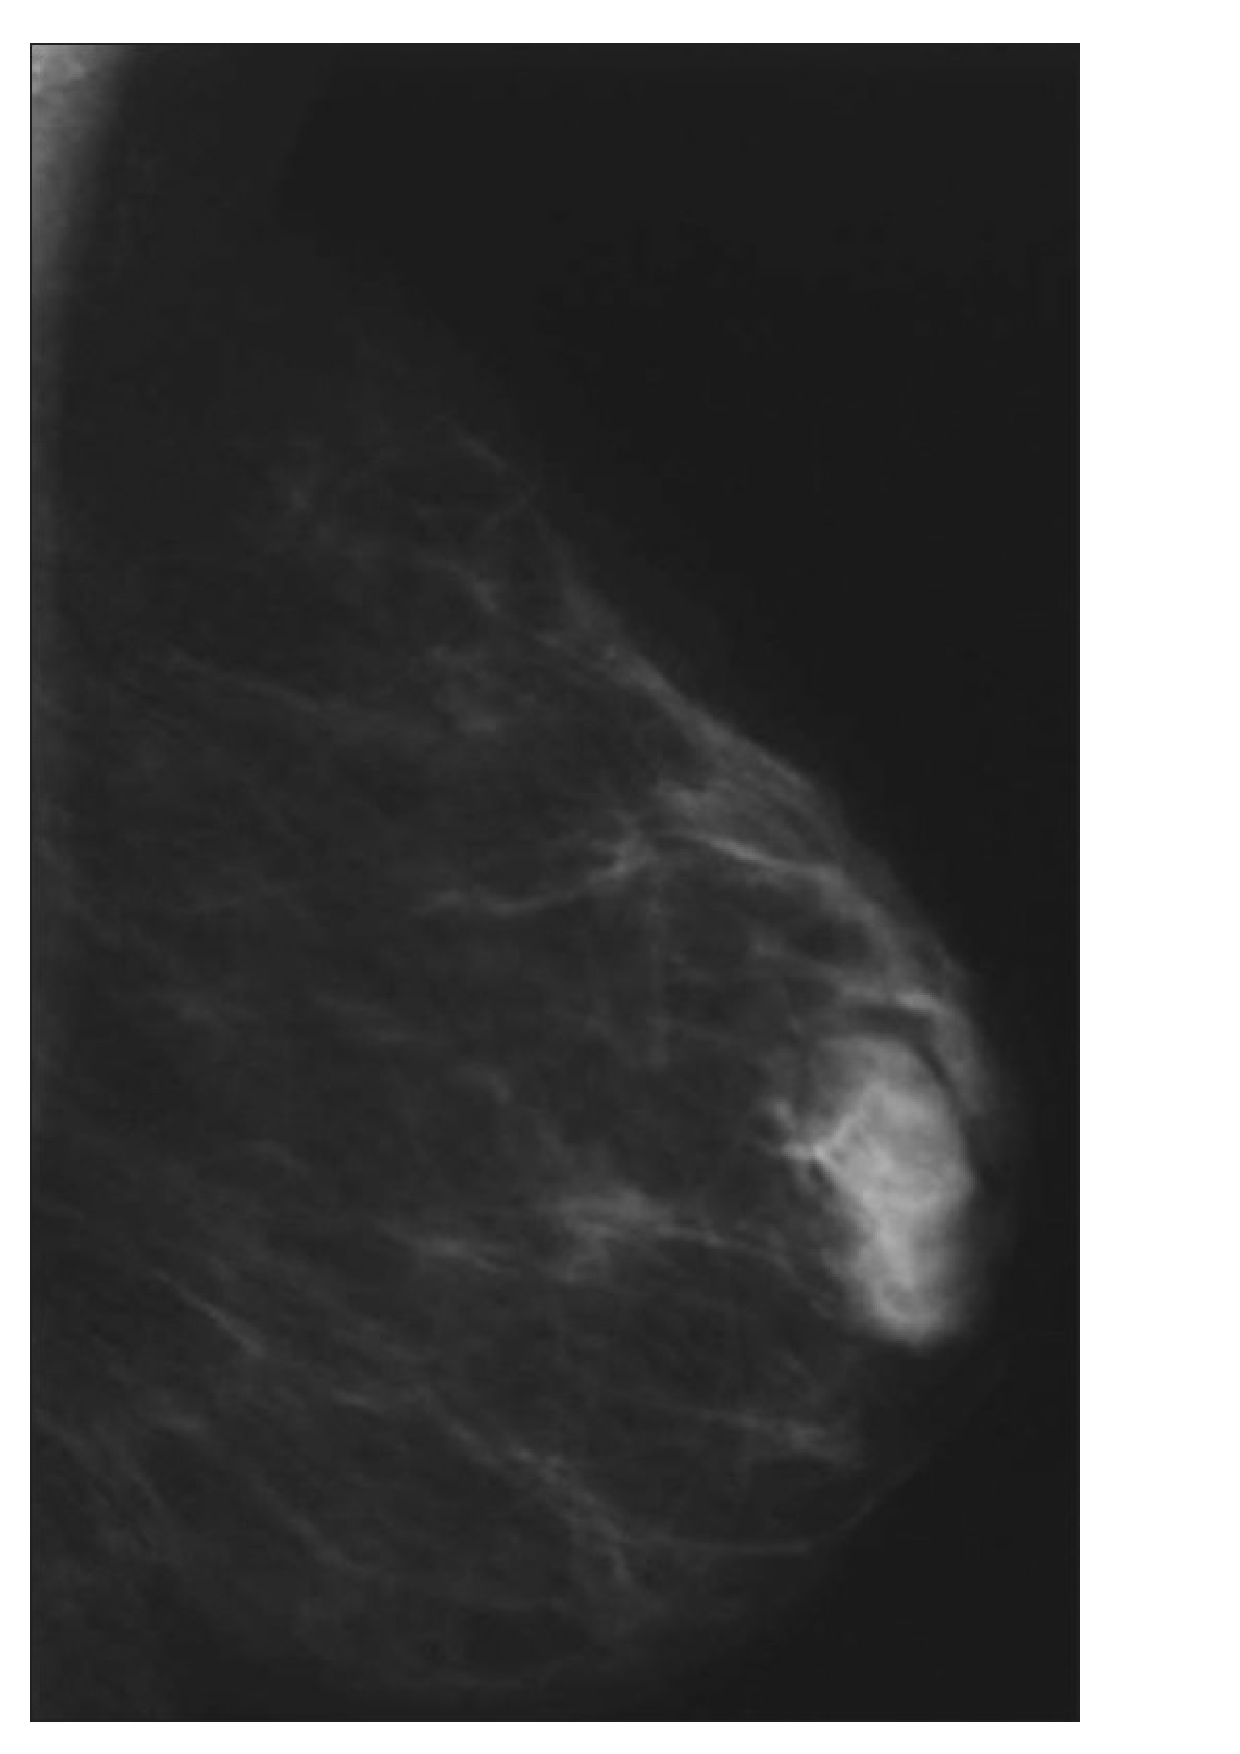
\includegraphics[width=3cm]{Figures/3715982_IJMPO-34-47-g001.png}
   		\captionof{subfigure}{Imagen original}
  	\end{minipage}
  \hspace{1pt}
   \begin{minipage}[t]{0.3\linewidth}  
   		\centering
        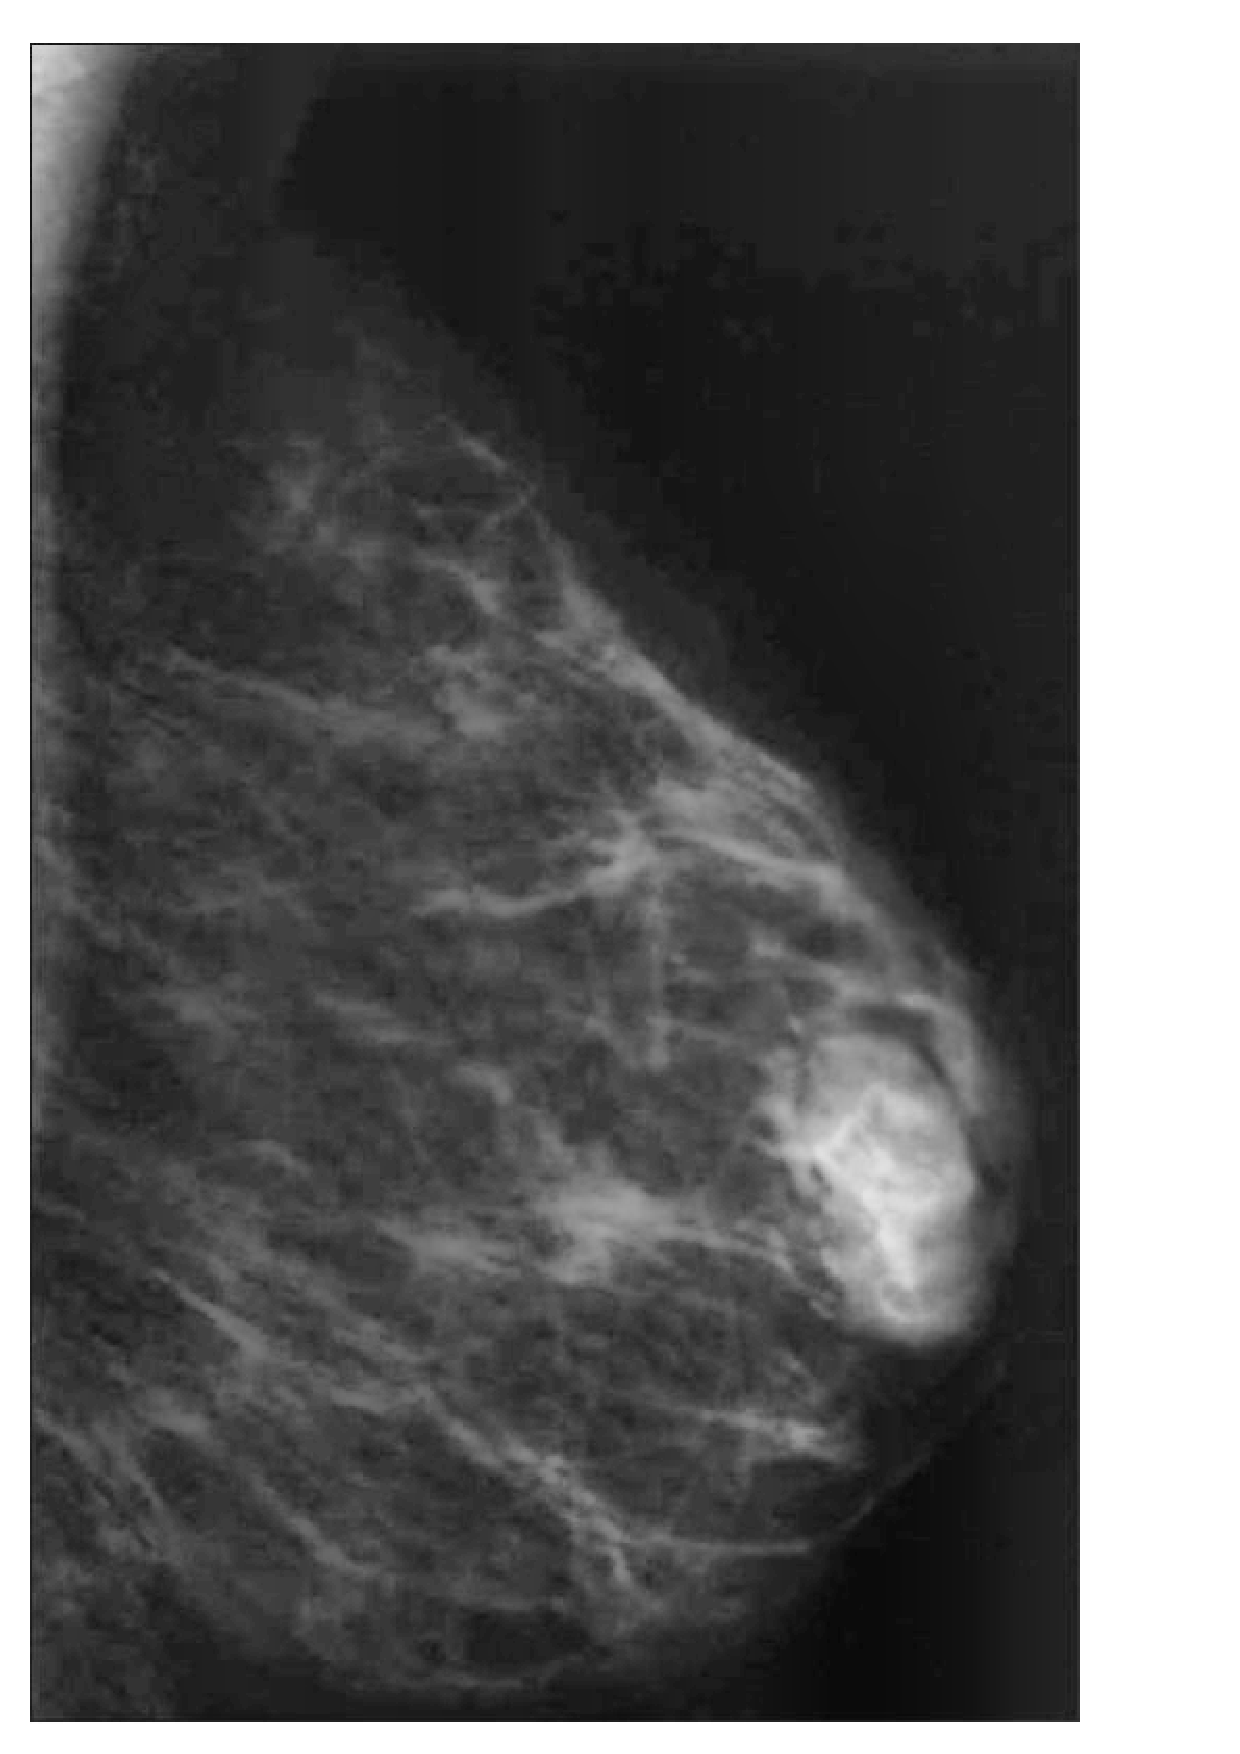
\includegraphics[width=3cm]{Figures/11608-3715982_IJMPO-34-47-g001.png}
   		\captionof{subfigure}{Imagen resultante. $SSIM=0.8032$ $\mathscr{H}=0.8549$}
  	\end{minipage}
   \begin{minipage}[t]{0.3\linewidth}  
   		\centering
        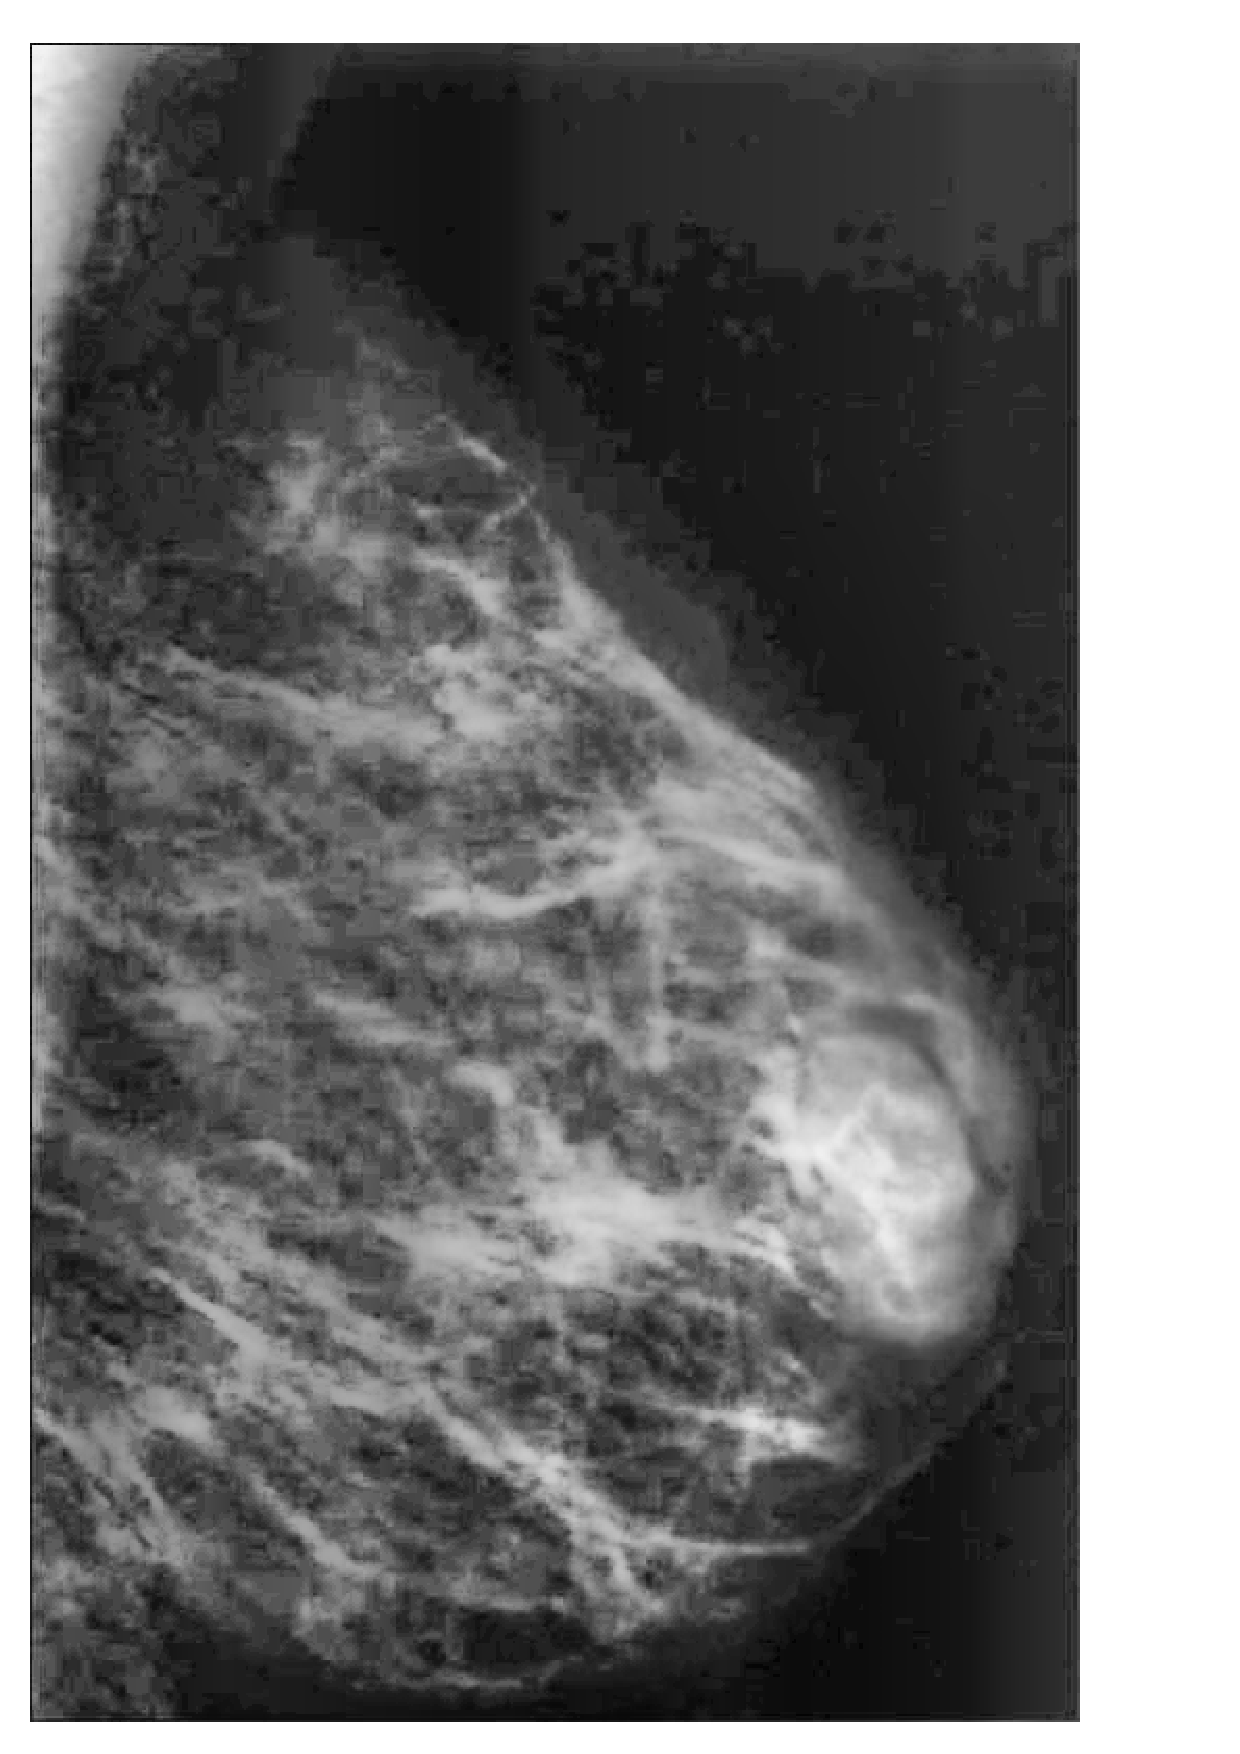
\includegraphics[width=3cm]{Figures/11806-3715982_IJMPO-34-47-g001.png}
   		\captionof{subfigure}{Imagen resultante. $SSIM=0.6059$ $\mathscr{H}=0.9163$}
  	\end{minipage}
  \vspace{0.5cm}
    \label{fig:resultado2}
  \captionof{figure}{Resultados de PSO-CLAHE multiobjetivo. }

\end{minipage}

\begin{minipage}[b]{1.0\linewidth}

   \begin{minipage}[b]{0.48\linewidth}  
   		
        \includegraphics[height=6cm , width=8.5cm]{Figures/pareto-chest.jpg}
   		\captionof{subfigure}{Frente Pareto de la \textbf{Fig. 2}}
  	\end{minipage}
   \hspace{1pt}
   \begin{minipage}[b]{0.48\linewidth}  
   		\centering
        \includegraphics[height=6cm, width=10cm]{Figures/pareto-mamografia.jpg}
   		\captionof{subfigure}{Frente Pareto de la \textbf{Fig. 3}}
  	\end{minipage}
  \vspace{0.5cm}
    \label{fig:resultado3}
  \captionof{figure}{Frentes Pareto para la \textbf {Fig. 2a} y la \textbf {Fig. 3a}. }

\end{minipage}


\twocolumn
\bibliographystyle{IEEEbib}
\bibliography{refs}



\end{document}
